% ------------------------------------------------------------------------------
% Este fichero es parte de la plantilla LaTeX para la realización de Proyectos
% Final de Grado, protegido bajo los términos de la licencia GFDL.
% Para más información, la licencia completa viene incluida en el
% fichero fdl-1.3.tex

% Copyright (C) 2012 SPI-FM. Universidad de Cádiz
% ------------------------------------------------------------------------------

En esta sección se recoge la arquitectura general del sistema de información, la parametrización del software base (opcional), el diseño físico de datos, el diseño detallado de componentes software y el diseño detallado de la interfaz de usuario.

\section{Arquitectura del sistema}
\subsection {Arquitectura física}
Las herramientas del proyecto OMI pueden ser dispuestas sobre diferente arquitecturas físicas. Por un lado se puede hacer uso 
del intérprete como una herramienta de un sistema operativo GNU/Linux, siguiendo así una arquitectura de escritorio. 
Por otro se puede usar el sistema en como una arquitectura cliente/servidor.

\subsubsection{Escritorio}
El cliente OMI puede ser utilizado en una arquitectura de escritorio, funcionando como un comando del sistema. Para ello solo se precisa de un PC con un sistema operativo GNU/Linux.

\subsubsection{Cliente/servidor}
El intérprete OMI puede ser usado en una arquitectura cliente/servidor, en la que hace de servidor. El servidor OMI espera una petición para un proceso de interpretación. Esta petición
contendrá el código fuente que se desea interpretar.

El servidor OMI procesa un código fuente para su interpretación devolviendo una estructura de datos en formato JSON que representa el árbol de nodos resultado del análisis léxico y sintáctico. 
Luego espera peticiones para resolver cada paso dentro del proceso de interpretación y devolver una estructura de datos en el mismo formato que representa qué ha ocurrido mediante el estado actual.

El sistema servidor es independiente del cliente en el sentido de que pueden usarse distintos clientes para el mismo servicio. El proyecto OMI presenta un cliente web llamado runTree 
que funciona en cualquier navegador moderno, no obstante se puede usar otra tecnología como cliente. 

Para ejecutar el sistema en una arquitectura cliente servidor se precisa de un equipo que tenga conexión a internet con un navegador web que hará de cliente. Por otro lado se necesita de un equipo servidor
que presente una alta disponibilidad. Este equipo dispondrá de un sistema GNU/Linux sobre el que se ejecutará el intérprete y un servidor web Apache que servirá de plataforma para dar el servicio web.

\subsection {Arquitectura lógica}
En esta sección se presenta la arquitectura del sistema. Se presentan 
dos niveles de organización la parte frontal (front-end) y la parte 
interna o motor (back-end). 

La parte frontal se encarga de analizar y procesar la entrada del usuario.
Una vez tratada la entrada, se pasa la ejecución a las estructuras que conforman 
el motor del sistema. Estas llevarán a cabo una serie de tareas que puden producir
un resultado que será enviado al frontal. La parte frontal mostrará 
los datos como salida del programa en un formato establecido.

\begin{center}
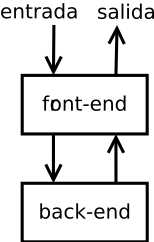
\includegraphics[scale=0.7]{design/dia/generic.png} 
\captionof{figure}{Arquitectura lógica}
\end{center}

Aunque bien se podría haber especificado otra capa correspondiente a la gestión de datos
llevada a cabo por las tablas de símbolos, esta se ha incluido en la parte del motor. Los datos que 
las tablas de símbolos tratan no mantienen persistencia, están muy ligados al proceso interno de 
interpretación y no representan los datos correspondientes al modelo de datos, sino que sirve para
referenciar componentes de la capa del motor de la aplicación.

\subsubsection{Frontal (front-end)}
El frontal del sistema se compone de un analizador léxico y un analizador sintáctico. 
Aunque es posible especificar reglas léxicas mediante reglas gramaticales, se ha separado el 
estos dos componentes por los siguientes motivos:

\begin{itemize}
\item La reglas lexicográficas suelen ser muy simples y para su descripción no se precisa de una 
notación tan compleja como las gramaticales.
\item Las expresiones regulares son más concisas y fáciles de entender que las gramáticas
\item A partir de expresiones regulares se puede describir analizadores léxicos eficientes.
\item Se modulariza el proceso en dos componentes con objetivos bien definidos. 
\end{itemize}

Además del analizador léxico y sintáctico el front-end contiene estructuras funcionales correspondientes
a la toma de datos de entradas y a la impresión de la salida. 

\paragraph {Analizador léxico}
El analizador léxico implementa una gramática de tipo 3 en la jerarquía de Chomsky (referencia: Compiladores y procesadores del lenguaje [José Antonio Jiménez Millán]), estas
se corresponden con las gramáticas regulares. 

Las gramáticas regulares, también llamadas gramáticas finitas, se pueden describir mediante expresiones regulares. 
Cada expresión regular denota un lenguaje $L(r)$. Una expresión regular se construye a partir de otras expresiones
más simples, utilizando un conjunto definidos de reglas. Estas reglas indican la manera de conseguir el conjunto 
$L(r)$ combinando de varias formas los lenguajes denotados por las subexpresiones de $r$. Las expresiones regulares
se pueden definir de una forma recursiva como sigue: 

\begin {enumerate}
\item $\epsilon$ es una expresión regular que denota el lenguaje que unicamente contiene la cadena vacía.
\item Si $a$ fuese un símbolo del alfabeto, entonces $a$ es una expresión regular que denota el lenguaje formado
por la cadena $a$.
\item Si $r$ y $s$ son dos expresiones regulares que denotan los lenguajes $L(r)$ y $L(s)$ respectivamente entonces:
\begin{itemize}
   \item $L(r|s)\ \rightarrow\ L(r)\ \cup\ L(s)$
   \item $L(rs) \ \rightarrow\ L(r)L(s)$
   \item $L(r*)\ \rightarrow\ (L(r))*$
   \item $L(r+)\ \rightarrow\ (L(r))+$
   \item $L(r?)\ \rightarrow\ \{\epsilon\}\ \cup\ L(r)$
   \item $L((r))\ \rightarrow\ (L(r))$
\end{itemize}
\end{enumerate}

Las gramáticas regulares pueden ser implementadas mediante un autómata finito. Un autómata finito se define formalmente como sigue:
$$AF = (S,\Sigma,\delta,S_0,F)$$

De forma que:
\begin{itemize}
\item $S$ es un conjunto de estados.
\item $\Sigma$ es el conjunto de símbolos que conforman el alfabeto.
\item $\delta$ es una función de transición tal que $(\delta\ :\ S\times\Sigma \rightarrow S)$. Donde para cada estado y según 
cada carácter de entrada del alfabeto le hace corresponder un nuevo estado.
\item $S_0$ es el estado inicial.
\item $F$ es un conjunto de estado finales.
\end{itemize}

El analizador léxico se corresponde con un autómata finito donde, al alcanzarse un estado final, se produce la generación de un token.
Un token es un elemento léxico con cierto valor para el lenguaje. Normalmente se corresponde con una cadena de
caracteres que se puede corresponder con una palabra reservada, un identificador, un número... Un token puede contener un 
valor. Los token son utilizados por el analizador sintáctico para llevar a cabo el procesamiento del código fuente. 

Las reglas lexicográficas a partir de las cuales se construye el analizador léxico son descritas junto la gramática, haciendo uso
de expresiones regulares y diagramas sintácticos.

\paragraph{Analizador sintáctico}
El analizador sintáctico implementa una gramática de tipo 2 en la jerarquía de Chomsky, esta se corresponden con las 
gramáticas independientes del contexto. Una gramática de este tipo, como su propio nombre indica, no depende del contexto para
su resolución, lo que origina que los recursos que permiten analizarlas sean relativamente eficientes y simples. Una gramática de
este tipo pueden ser analizadas mediante algoritmos con un orden $O(n^3)$ donde $n$ es el tamaño de la entrada. No obstante existen 
un subconjuntos de este tipo de gramáticas como las $LL(k)$ y $LR(k)$ que pueden ser analizados en tiempo $O(n)$. Estos últimos son los
comúnmente utilizados en los lenguajes de programación.

En el análisis sintáctico se pueden utilizar métodos descendentes o ascendentes, en función de cómo se genera el árbol sintáctico. 

Los métodos de análisis descendentes tienen como objetivo construir el árbol de derivación desde la raíz hacia las hojas. Normalmente se
utilizan analizadores del tipo $LL$ dado que la entrada es tratada desde la izquierda y las reglas de producción también desde la izquierda.
Estos tipos de analizadores tienen el problema de la incertidumbre, debido a que dado un símbolo no terminal debe determinar qué regla de derivación aplicar. 
La incertidumbre puede ser reducida mediante métodos como el retroceso o la predicción.
 
Los métodos de análisis de ascendentes pretenden construir el árbol de derivación o de sintaxis desde las hojas hacia la raíz. Para este tipo normalmente se utiliza 
analizadores del tipo $LR$ dado que la entrada es tratada desde la izquierda, mientras que las reglas de producción son tratadas desde la derecha. Este tipo de
analizadores reducen la incertidumbre dado que se parte de una una regla de derivación para obtener el símbolo no terminal que se corresponde a la misma. 

Para el lenguaje tratado en este proyecto se tomará un analizador sintáctico ascendente $LR$, dado que es uno de los más utilizados, son eficientes y 
existen herramientas que permiten su generación automática a partir de la descripción de la gramática. 

Las gramáticas libres de contexto son analizadas mediante un autómata de pila. La configuración en un momento dado del analizador se corresponde con el contendido de la pila y el resto de la 
entrada que aún está por analizar. La entrada estará constituida por tokens obtenidos por el analizador léxicos, teóricamente estos serán almacenados en una estructura de buffer, pero 
en la práctica estos son generados bajo demanda por el analizador léxico. En la pila se irá almacenando una serie de estados en función del procesamiento realizado sobre la cadena de entrada. 
El autómata puede llevar a cabo dos operaciones:

\begin{description}
\item[Desplazar:] Consiste en sacar del buffer de entrada un símbolo terminal e introducir el estado correspondiente en la pila.
\item[Reducir:] Consiste en reducir $n$ estados del tope de la pila al estado correspondiente, según las reglas de producción.
\end{description}

El análisis finaliza cuando se produce un estado de aceptación o de error. 

En la práctica este tipo de analizador sintáctico se implementa mediante un programa monitor que encierra la lógica descrita, un buffer de entrada en el que se almacenan
los tokens, una pila que almacena los estados producidos, y dos tablas. La primera tabla guardará las acciones y determina, para el estado actual y el primer símbolo del buffer, 
la acción a realizar (desplazar o reducir). La otra tabla, la tabla de saltos, es utilizada tras llevarse a cabo una de reducción, y determina a partir del estado en el tope de la pila
tras la reducción y la regla que se utilizó para la misma, el siguiente estado a introducir en la pila. 

\begin{center}
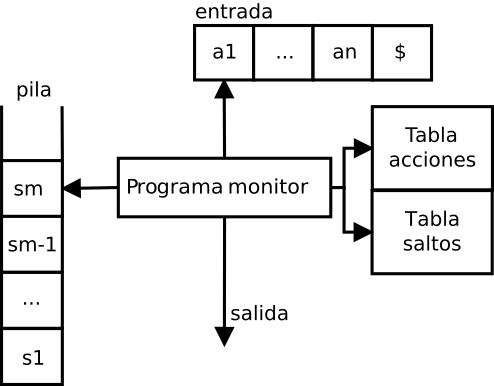
\includegraphics[scale=0.7]{design/dia/asd.png} 
\captionof{figure}{Arquitectura analizador sintáctico}
\end{center}

Por cada reducción que se lleve a cabo se creará un nodo del árbol sintáctico. De esta forma el árbol es creado desde las hojas hacia la raíz. Cada nodo encierra un significado semántico que 
será llevado a cabo cuando se ejecuten. Estos nodos constituyen a su vez el motor, o back-end, del sistema.

\paragraph{Mecanismos de entrada/salida}
En el nivel de front-end también se dan los diferentes componentes para capturar la entrada del usuario, así como para facilitar la salida que produce en sistema.

La entrada más común supondrá código fuente que será interpretado y ejecutado. Este se podrá dar de varias formas:

\begin{itemize}
\item Mediante la entrada estándar del sistema.
\item Contenido en fichero.
\item Mediante un intérprete de línea.
\end{itemize}

Es posible que se den datos de entrada que no sean código fuente, como por ejemplo, una extensión que debe ser cargada, la opción de mostrar ayuda ...

Por otro lado los datos de salida que produce el programa normalmente serán volcados en la salida estándar sistema en forma de cadenas de caracteres. 
Esta será el resultado visual de la interpretación del código fuente, aunque es posible que un determinado código fuente no produzca salida de este tipo. 

El programa debe ser capaz de procesar los errores y mostrarlos por la salida de errores del sistema. Para ello debe controlar las líneas y ficheros procesados en cada
momento. Los errores pueden ser de diferente tipos:

\begin{itemize}
\item Errores léxicos.
\item Errores sintácticos.
\item Errores semánticos.
\end{itemize}

Además los errores pueden presentar diferente grado:

\begin{description}
\item [Avisos:] Informan de que algún recurso del lenguaje no se utiliza de la forma habitual, y aunque no se produce un error como tal, puede suponer un error de codificación.
\item [Normales:] No finalizan la ejecución del código fuente pero provocan que la sentencia en la que sucede no se pueda ejecutar.
\item [Críticos:] Finalizan la ejecución del código fuente.
\end{description}

\subsubsection{Motor (back-end)}
El motor del sistema lo conforman los nodos creados mediante el análisis sintáctico. Estos nodos se denominan nodos ejecutables, dado que su procesamiento conlleva la realización operacional
de la semántica que encierran. Los nodos ejecutables se categorizan según el tipo de operaciones que conlleva su ejecución, así existen nodos aritméticos, lógicos, de control de flujo, 
de definiciones... 

El sistema presenta una jerarquía de nodos ejecutables que establece la naturaleza de los mismos, dotándolos de características de una forma general y que serán concretadas en los niveles más
bajos de la jerarquía. Se presenta de esta forma, nodos ejecutable genéricos como expresiones, referencias, imprimibles....

El procesamiento de un nodo ejecutable, que fue creado a partir del análisis sintáctico, puede originar la creación de otros nodos ejecutables, a estos 
últimos se les denominará nodos ejecutables dinámicos. Un nodo dinámico es creado y referenciado por una estructura de datos denominada tabla de símbolos. 
Esta estructura también es considerada un componente del motor del sistema.

Los nodos ejecutables presentan dos niveles de procesamiento semántico: la inicialización y la ejecución. Además también se ha de controlar cómo estos son creados y eliminados de 
forma dinámica en la tabla de símbolos. 



\paragraph{Inicialización}
Todo nodo ejecutable se inicializa a partir de otros nodos ejecutable sobre los que operará. Normalmente estos nodos se corresponderán con los hijos del nodo en cuestión en el árbol sintáctico. 

La inicialización de un nodo ejecutable se lleva a cabo durante la creación del árbol sintáctico, por tanto los nodos se inicializan de una forma ascendente, es decir,
antes los nodos hijos que los padre.

Durante la inicialización se lleva a cabo algunas comprobaciones de tipos, asignaciones y otras operaciones. No obstante, todo proceso que se lleve a cabo durante la
inicialización debe ser independiente de la ejecución. Se ha de tener en cuenta que un nodo ejecutable sólo se inicializa una vez, y sin embargo se puede ejecutar varias
veces, siendo esta última dependiente del estado en un momento dado. Se puede decir pues que la inicialización tiene un carácter estático.

\paragraph{Ejecución}
Una vez generado el árbol sintáctico, lo que conlleva la inicialización de los nodos ejecutables que lo componen, se procede a la ejecución del mismo. La ejecución comienza desde el 
nodo raíz hacia las hojas, se hace pues un recorrido del árbol en profundidad.

La ejecución de un nodo es iniciada normalmente desde su nodo padre, y generalmente conlleva la ejecución de sus nodos hijos antes de proceder a su propia ejecución. Así por ejemplo 
la ejecución de un nodo suma conllevará el cálculo del lado izquierdo de la expresión, lo que se corresponde con la ejecución uno de sus nodos hijo, luego se calculará
el lado derecho, correspondiente a la ejecución del otro nodo hijo, para, una vez ejecutados sus hijos (los operandos), proceder al cálculo de la suma, lo que se corresponde 
con su propia ejecución. 

Durante la ejecución de un nodo ejecutable lo normal es que primero se resuelvan los nodos referencias, aquellos que se corresponden con nodos dinámicos de tipos no definidos. Estos 
nodos referencian a otros nodos creados dinámicamente en la interpretación y que se encuentran accesibles desde la tabla de símbolos. Algunos nodos referencias, 
también denominados nodos de expresiones no definidas, son los correspondientes a: variables, funciones u clases de objetos. Una vez se ha obtenido el nodo al que estos referencian, 
se procede con la ejecución como si los nodos obtenidos fueran los hijos del nodo en proceso.

Aunque la ejecución del árbol se hace inicialmente con un recorrido en profundidad existen nodos que rompen esta secuencia, haciendo que la ejecución pase a nodos específicos 
o repitiendo la ejecución de varios de sus hijos. Cabe decir que una vez se salte la secuencia de ejecución el recorrido seguirá siendo en profundidad. Estos nodos 
se corresponden con sentencias de control de flujo, llamadas a funciones, etc.

El resultado de ejecutar un nodo no tiene por que ser estático, dependiendo en gran medida del contexto, es decir, del estado de la tabla de símbolos. Se puede decir pues que la 
ejecución de un nodo tiene un carácter dinámico dependiente de la tabla de símbolos.

\paragraph{Tabla de símbolos}
La tabla de símbolos es una estructura de datos que almacena referencias a nodos creados dinámicamente en el proceso de interpretación. Estos nodos serán creados en la 
ejecución del árbol de sintáctico y serán accedidos desde la ejecución de determinados nodos en la resolución de referencias. 

Las tablas de símbolos se componen de pares donde el primer elemento es un identificador que nomina al símbolo y el segundo elemento es una referencia al nodo ejecutable. 

Aunque en una tabla de símbolos es posible guardar referencias a cualquier nodo se mantiene diferentes tipos tablas de símbolos según la naturaleza de los nodos a los que se
referencian. Esto hace posible que se puedan repetir identificadores para distintos tipos de nodos como variables, funciones o clases.

Dos identificadores que pueden estar en la misma tabla de símbolos o distintas, pueden referenciar al mismo nodo. El propio nodo debe ser capaz de guardar cuantas referencias al 
mismo tiene. Esto se hace por criterios de optimización, para la reutilización de datos y para realizar una eliminación del nodo de una forma segura cuando sea necesario.

Las tablas de símbolos pueden quedar organizadas en niveles, aunque únicamente un nivel, el actual en un momento dado, es el que se utilizará para la resolución de referencias.
Esto hace posible definir diferentes ámbito para el acceso a determinados símbolos. Los niveles quedan dispuestos en una estructura de pila, de forma que el nivel actual es
la cima de la pila. Una vez un nivel es eliminado de la pila se eliminan todas las referencias del mismo y el nivel anterior queda en la cima y por tanto es considerado el nivel actual.

Existen nodos que presentan sus propias tablas de símbolos, esto hace que muchas definiciones sean internas al mismo. Por ejemplo las clases de objetos mantienen sus propias tablas
de símbolos para referencias los métodos y atributos, y los arrays presentan una tabla de símbolos para guardar las claves y sus valores. Es común que en la ejecución 
de uno de estos nodos se sustituya la tabla de símbolos en uso por la del nodo en cuestión.

La tabla de símbolo es una estructura de datos que forma parte del motor de la aplicación dado que gestiona y almacena datos presentes en este nivel. 

\paragraph{Eliminación de referencias}
Los nodos creados de forma dinámica por el proceso de interpretación deben ser eliminados cuando ya no se precisen de ellos. Por ejemplo cuando se produce una asignación destructiva. Como
los nodos creados de forma dinámica son reutilizados y pueden ser referenciados por más de un símbolo se ha de controlar que no exista ninguna referencia al mismo 
antes de proceder a su eliminación. Así cada nodo guarda el número de referencias al mismo.

Los nodos correspondientes al árbol sintáctico nunca serán eliminados durante la ejecución y no será hasta la finalización del programa hasta que se proceda a la liberación de los recursos 
que consumen.





\subsubsection{runTree}
runTree es un sistema que hace de cliente del intérprete OMI, cuando este funciona como servidor. Se encarga de llevar a cabo peticiones para navegar por el proceso de interpretación de un código
fuente dado. 

El cliente runTree presenta una arquitectura interna en dos capas al igual que el intérprete. El backend de este se comunica con el frontend del intérprete cuando funciona de servidor

\begin{center}
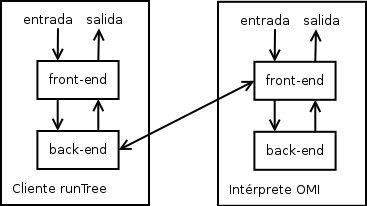
\includegraphics[scale=0.7]{design/generic_cliente_servidor.png} 
\captionof{figure}{Arquitectura runTree}
\end{center}

El frontend del cliente runTree lo componen elementos relacionados con la interfaz del usuario. Captura eventos de esta y lo envía al backend para su procesamiento, a su vez representa los datos que recibe del backend. 

El backend del cliente runTree lo componen elementos que guardan el estado interno del proceso de interpretación. Normalmente estos elementos son inicializados mediante datos que recibe del servidor como fruto de 
una petición.


\section{Diseño de la gramática}
En esta sección se presenta la gramática del lenguaje, para ello 
se procede a una descripción de las reglas gramaticales
 mediante el lenguaje EBNF (Extended Backus–Naur Form) 
usado para expresar gramáticas libres de contexto. Además cada regla se acompaña de un
diagrama sintáctico o diagrama de carril. 

Una gramática $G$ se define formalmente como sigue:

$$G = (V_t,V_n, P, S)$$

De forma que:

\begin{description}
\item[$V_t$] es un conjunto finito de símbolos terminales
\item[$V_n$] es un conjunto finito de símbolos no terminales
\item[$P$] es un conjunto finito de reglas de producción
\item[$S\ \epsilon\ V_n$] es el símbolo inicial
\end{description}

Las reglas de producción de una gramática libre de contexto tiene la forma siguiente forma:

$$V_n\ \rightarrow\ (V_t\ \cup\ V_n)^*$$ 

La gramática libre de contexto abordada tiene como símbolo inicial 
el no terminal $program$. Se comienza pues describiendo las reglas de producción 
relacionadas con este símbolo, siguiendo con las reglas de producción derivadas 
de esta. 

Las reglas de producción se organizan en niveles como sigue:

\begin{center}
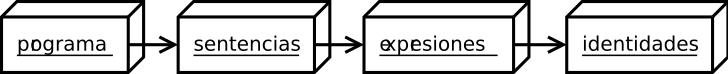
\includegraphics[scale=0.7]{design/diagram/omi.png} 
\captionof{figure}{Niveles reglas de producción}
\end{center}

Estos niveles son dados a partir del nivel de abstracción del significado 
semántico que encierran las reglas de producción contenidas en los mismos.

Las reglas de producción correspondientes al nivel de programa 
son las más genéricas y se valen de las de la siguiente nivel para 
su definición. Estas definen el programa como una secuencia de
sentencias. La gramática descrita contempla el programa vacío, es decir,
el programa que no contiene ninguna sentencia.

Las reglas de producción del nivel de sentencia se definen a 
partir de expresiones o de otras sentencias. Una sentencia contiene un significado semántico
operativo de valor para el programa. Cabe decir que una expresión por si sola 
puede constituir una sentencia. La gramática expuesta describe la sentencia
vacía, esta es una sentencia que no tienen ningún significado semántico.

Las expresiones son la unidad mínima con significado semántico atribuido por 
el lenguaje. La mayoría de expresiones se definen a partir de identidades, 
sin embargo algunos tipos de expresiones, como las funciones, pueden formarse
a partir de reglas de más alto nivel de abstracción semantica. Por otro lado las 
reglas de producción correspondiente a las expresiones están organizadas en niveles según
la prioridad atribuida en su resolución.

Las identidades son reglas de producción atómicas, componiéndose únicamente de símbolos no terminales. 
Tienen un significado semántico asociado de forma directa. Normalmente este valor viene dado por 
el análisis léxico.  
 
% ----------------------------------------------------------------------
\subsection{Programa}
\begin{multicols}{2}
\begin{lstlisting}[style=nonumbers]
program  ::=  stmts
            | empty
\end{lstlisting}  
\columnbreak
\begin{center}
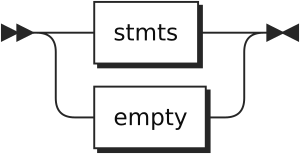
\includegraphics[scale=0.7]{design/diagram/program.png} 
\captionof{figure}{Gramática programa}
\end{center}
\end{multicols}
% ----------------------------------------------------------------------
\subsection{Sentencias}
\subsubsection{Secuencia de sentencias}
\begin{multicols}{2}
\begin{lstlisting}[style=nonumbers]
stmts    ::=   stmt ";" stmts
            |  stmt ";"?
            |  stmtb 
            |  label stmts
            |  ";"
\end{lstlisting}  	
\columnbreak
\begin{center}
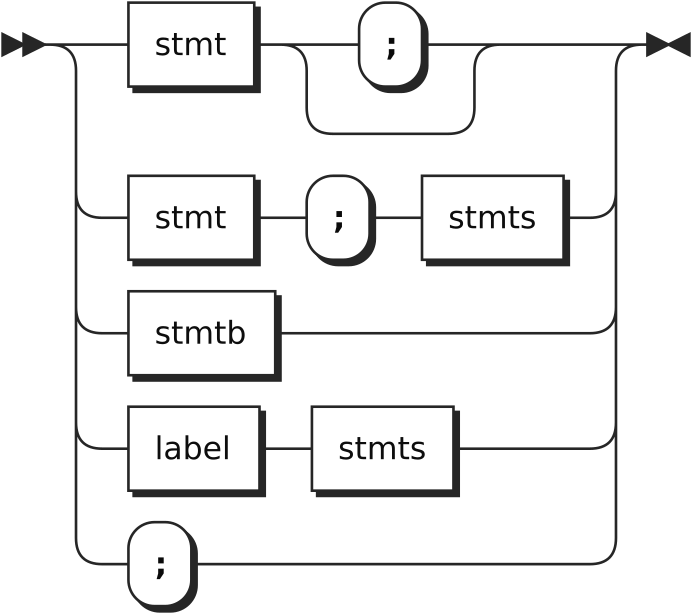
\includegraphics[scale=0.65]{design/diagram/stmts.png} 
\captionof{figure}{Gramática sentencias}
\end{center}
\end{multicols}

\subsubsection{Sentencia de bloque}
\begin{multicols}{2}
\begin{lstlisting}[style=nonumbers]
stmtb ::=   if
         |  while
         |  dowhile
         |  for
         |  foreach
         |  break
         |  switch
         |  iloop
         |  trycatch
         |  class
         |  with
\end{lstlisting}  	
\columnbreak
\begin{center}
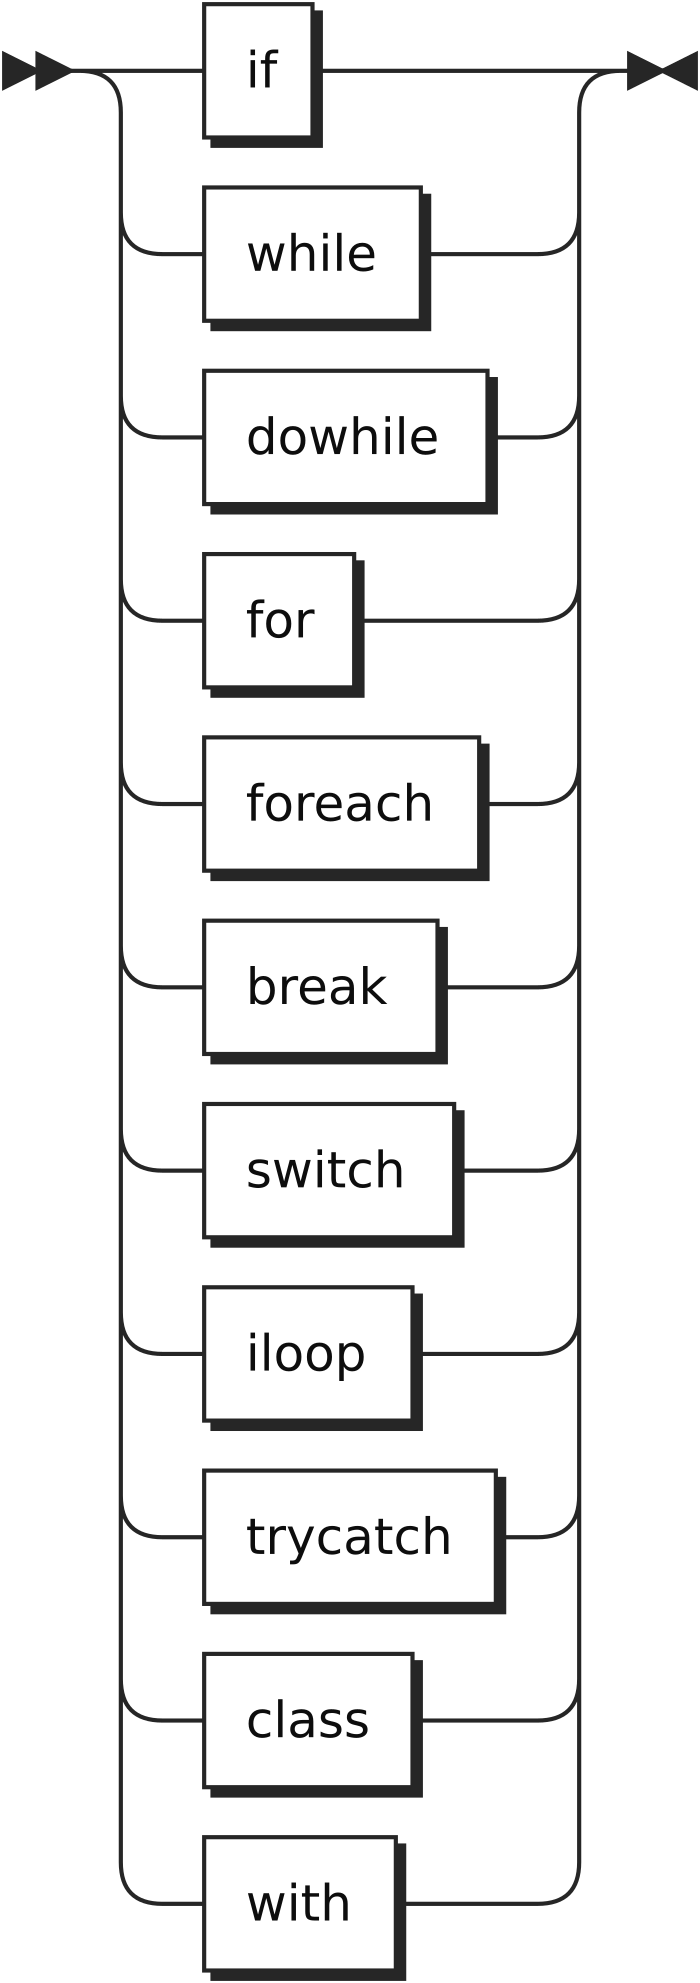
\includegraphics[scale=0.7]{design/diagram/stmtb.png} 
\captionof{figure}{Gramática sentencias de bloque}
\end{center}
\end{multicols}
\paragraph{Sentencia de control: if}
\begin{lstlisting}[style=nonumbers,
    basicstyle=\tiny, %or \small or \footnotesize etc.
]
if ::= "if" exp ("{" stmts? "}" | stmt ";" | stmtb) elif* ("else" ("{" stmts? "}" | stmt ";" | stmtb))?

elif ::=  "elif" exp ( "{" stmts? "}" | stmt ";" | stmtb ) 
\end{lstlisting}  	
\begin{center}
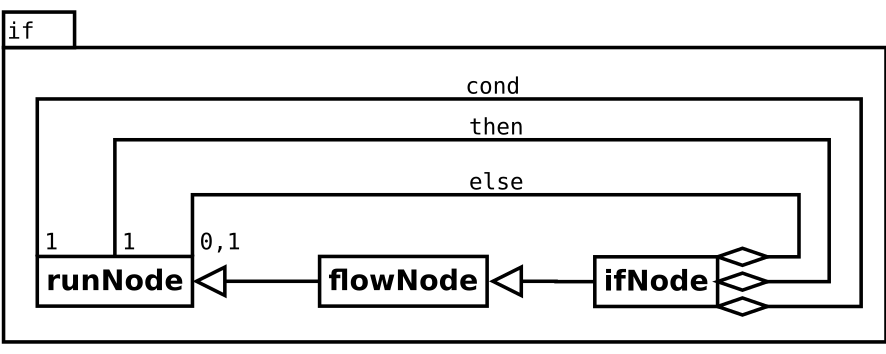
\includegraphics[scale=0.5]{design/diagram/if.png} 
\captionof{figure}{Gramática if}
\end{center}
\begin{center}
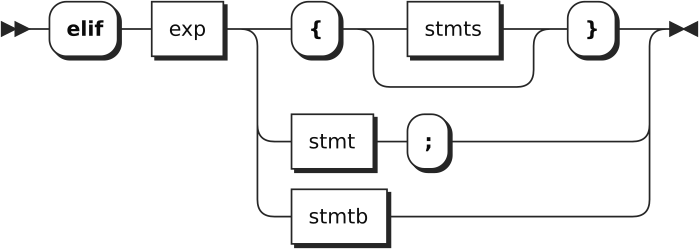
\includegraphics[scale=0.5]{design/diagram/elif.png} 
\captionof{figure}{Gramática elif}
\end{center}

\paragraph{Sentencia de control: while}
\begin{multicols}{2}
\begin{lstlisting}[style=nonumbers,
    basicstyle=\tiny]
while ::= 
   "while" exp ("{" stmts? "}" | stmt ";" | stmtb)
\end{lstlisting}  	
\columnbreak
\begin{center}
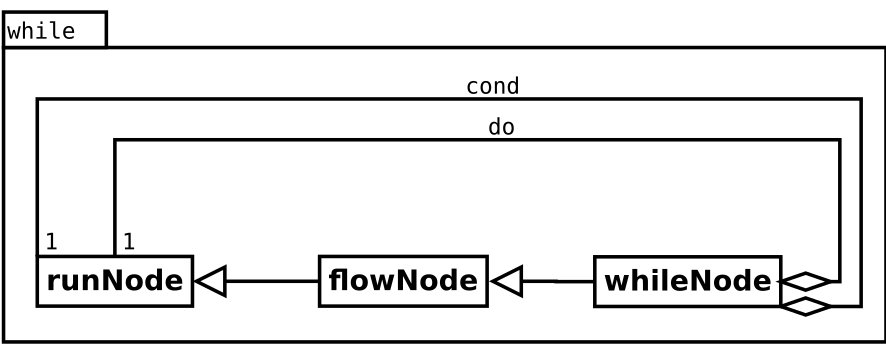
\includegraphics[scale=0.5]{design/diagram/while.png} 
\captionof{figure}{Gramática while}
\end{center}
\end{multicols}

\paragraph{Sentencia de control: do...while}
\begin{lstlisting}[style=nonumbers]
dowhile ::=  "do" ( "{" stmts? "}" | stmt ";" | stmtb ) "while" exp ";"
\end{lstlisting}  	
\begin{center}
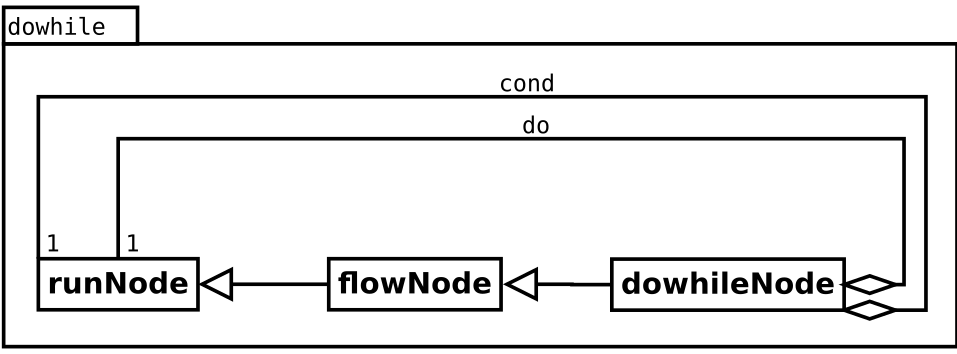
\includegraphics[scale=0.5]{design/diagram/dowhile.png} 
\captionof{figure}{Gramática dowhile}
\end{center}

\paragraph{Sentencia de control: for}
\begin{lstlisting}[style=nonumbers]
for ::= "for" "("? exp? ";" exp? ";" exp? ")"? 
   ( "{" stmts? "}"  | stmt ";" | stmtb )
\end{lstlisting}  	
\begin{center}
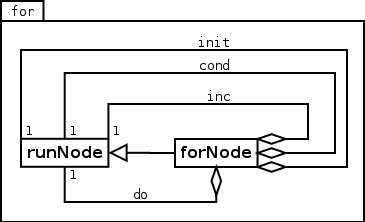
\includegraphics[scale=0.4]{design/diagram/for.png} 
\captionof{figure}{Gramática for}
\end{center}
\paragraph{Sentencia de control: forearch}
\begin{lstlisting}[style=nonumbers,basicstyle=\tiny]
foreach ::= 
   "for" "("?(id (":" id)? "in" exp | exp "as" id (":" id)?)")"? ("{" stmts? "}" | stmt ";" | stmtb)
\end{lstlisting}  	
\begin{center}
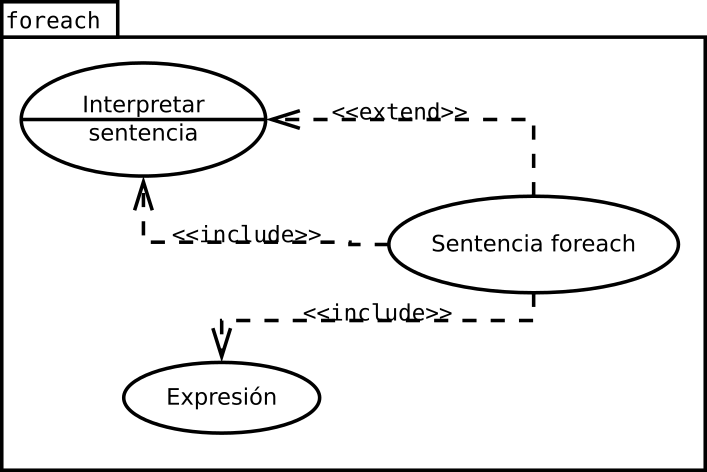
\includegraphics[scale=0.4]{design/diagram/foreach.png} 
\captionof{figure}{Gramática foreach}
\end{center}
\pagebreak
\paragraph{Sentencia de control: switch}
\begin{lstlisting}[style=nonumbers]
switch ::= "switch" "(" exp ")" "{" cases? "}"

cases ::= "case" exp ":" ( stmts cases | stmts | cases )
   |  "default" ":" stmts
\end{lstlisting}  	
\begin{center}
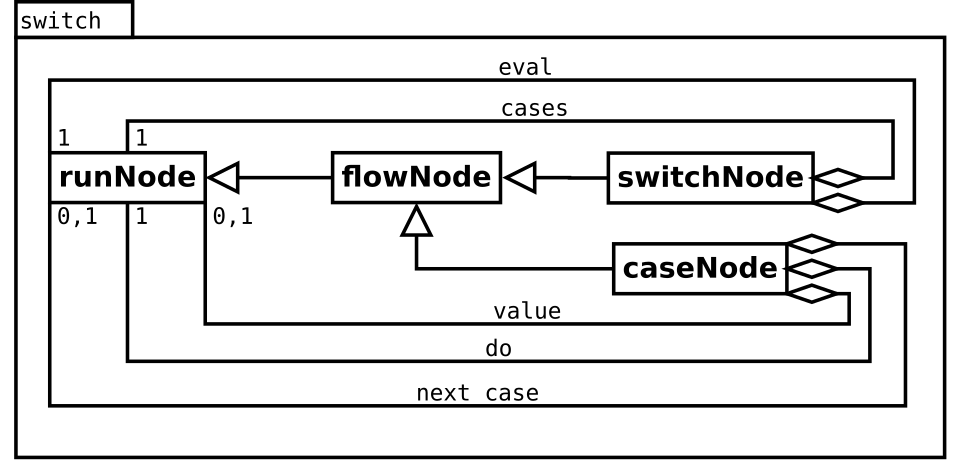
\includegraphics[scale=0.37]{design/diagram/switch.png} 
\captionof{figure}{Gramática switch}
\end{center}
\begin{center}
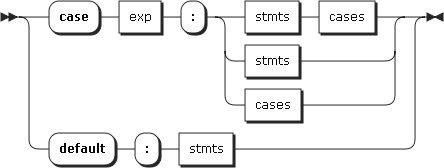
\includegraphics[scale=0.37]{design/diagram/cases.png} 
\captionof{figure}{Gramática cases}
\end{center}

\paragraph{Sentencia de control: iloop}
\begin{lstlisting}[style=nonumbers,basicstyle=\tiny]
iloop ::= "$" "(" exp ( "as" id (":" id)? )? ("," exp )? ")" ( "{" stmts? "}" | stmt ";" | stmtb )

iloop_access ::=  "$"
               |  "$" "{" NUM "}"
\end{lstlisting}  	
\begin{center}
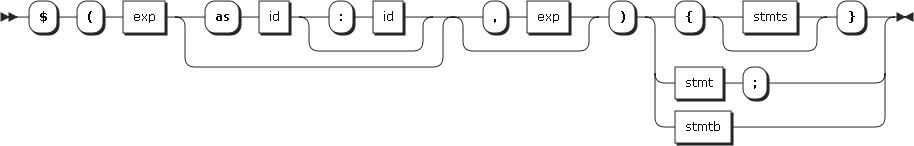
\includegraphics[scale=0.37]{design/diagram/iloop.png} 
\captionof{figure}{Gramática iloop}
\end{center}
\begin{center}
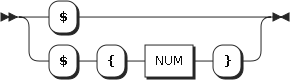
\includegraphics[scale=0.37]{design/diagram/iloop_access.png} 
\captionof{figure}{Gramática acceso iloop}
\end{center}

\paragraph{Sentencia de control: try...catch}

\begin{lstlisting}[style=nonumbers,basicstyle=\tiny]
trycatch ::= 
 "try" ( "{" stmts? "}" | stmt ";" | stmtb ) catch "(" id ")" ( "{" stmts? "}" | stmt ";" |  stmtb )
\end{lstlisting}  	
\begin{center}
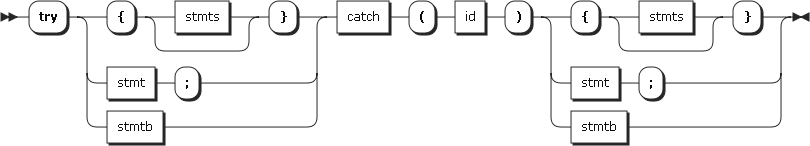
\includegraphics[scale=0.37]{design/diagram/trycatch.png} 
\captionof{figure}{Gramática trycatch}
\end{center}

\paragraph{Sentencia de control: with}
\begin{multicols}{2}
\begin{lstlisting}[style=nonumbers,basicstyle=\tiny]
with ::= 
 "with" exp ( "{" stmts? "}" | stmt ";" | stmtb )
\end{lstlisting}  	
\columnbreak
\begin{center}
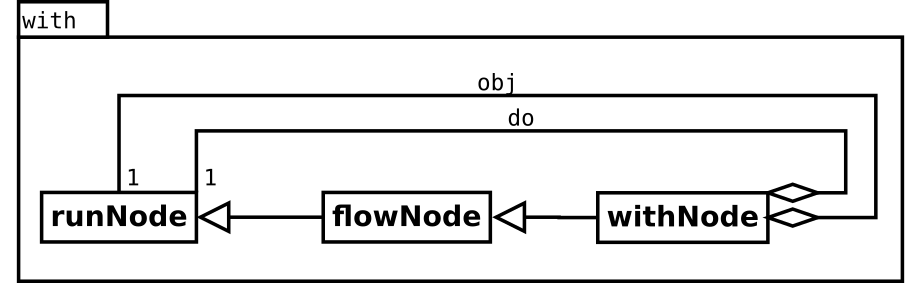
\includegraphics[scale=0.4]{design/diagram/with.png} 
\captionof{figure}{Gramática with}
\end{center}
\end{multicols}


\subsubsection{Sentencia simple}
\begin{multicols}{2}
\begin{lstlisting}[style=nonumbers]
stmt  ::=   exp
         |  "<<" exp
         |  ">>" ("[" exp "]")? id
         |  "goto" exp
         |  "include" exp
         |  "return" exp?
         |  "sleep" exp 
         |  "load" exp 
         |  "typeof" id 
         |  "datinfo" exp
         |  "exit"
         |  "throw" exp
         |  "global" identity
         |  "break" num? ";"
         |  "continue" num? ";"
\end{lstlisting}  	
\columnbreak
\begin{center}
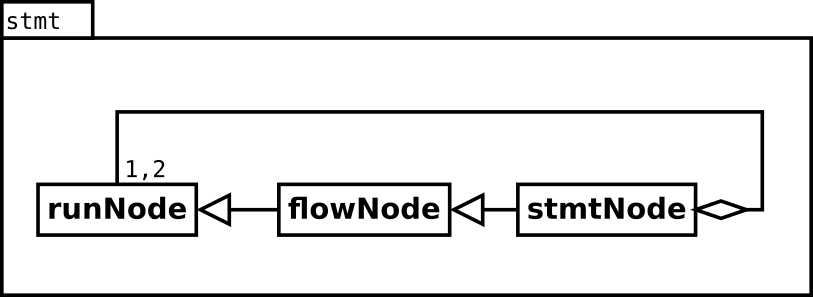
\includegraphics[scale=0.6]{design/diagram/stmt.png} 
\captionof{figure}{Gramática stmt}
\end{center}
\end{multicols}

\subsubsection{Etiquetas}
\begin{multicols}{2}
\begin{lstlisting}[style=nonumbers]
label ::=   id ":"
\end{lstlisting}  	
\columnbreak
\begin{center}
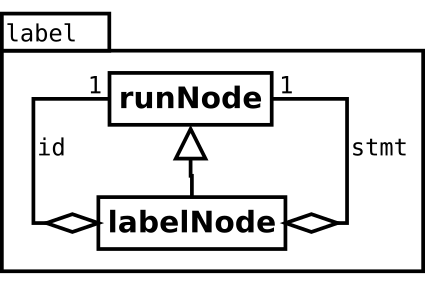
\includegraphics[scale=0.7]{design/diagram/label.png} 
\captionof{figure}{Gramática etiquetas}
\end{center}
\end{multicols}
\pagebreak
\subsubsection{Nombres de espacios}
\begin{multicols}{2}
\begin{lstlisting}[style=nonumbers, basicstyle=\tiny]      
namespace ::=  namespace "::" id
            |  id "::" id
            |  "parent" "::" id
            |  "static" "::" id
\end{lstlisting}  
\columnbreak	
\begin{center}
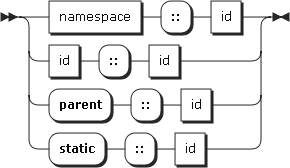
\includegraphics[scale=0.4]{design/diagram/namespace.png} 
\captionof{figure}{Gramática nombres  de espacios}
\end{center}
\end{multicols}
\subsubsection{Clases}
\begin{lstlisting}[style=nonumbers]
class ::= "class" id ("extends" id )? "{" class_stmts? "}"
\end{lstlisting}  	
\begin{center}
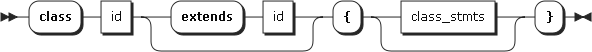
\includegraphics[scale=0.6]{design/diagram/class_gramatic.png} 
\captionof{figure}{Gramática clases}
\end{center}
\paragraph{Métodos y atributos}
\begin{lstlisting}[style=nonumbers]
class_stmts ::= 
   (("static"|"private"|"private" "static"|"static" "private")? (function|id|assig))*

\end{lstlisting}  	
\begin{center}
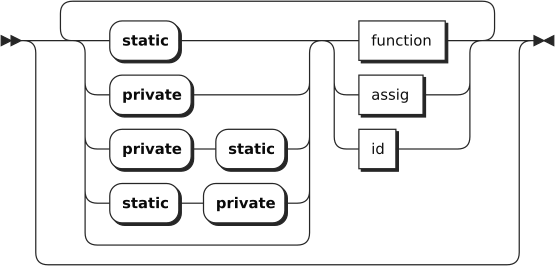
\includegraphics[scale=0.7]{design/diagram/class_stmts.png} 
\captionof{figure}{Gramática métodos y atributos}
\end{center}
% ----------------------------------------------------------------------
% ----------------------------------------------------------------------
\subsection {Expresiones}
\begin{multicols}{2}
\begin{lstlisting}[style=nonumbers]      
exp ::= op1
\end{lstlisting}  
\columnbreak	
\begin{center}

\includegraphics[scale=0.5]{design/diagram/exp.png} 
\captionof{figure}{Gramática expresiones}
\end{center}
\end{multicols}
\subsubsection{Operadores lógicos}
\paragraph{Or lógico}
\begin{multicols}{2}
\begin{lstlisting}[style=nonumbers]      
op1 ::=  op1 ( "||" | "or" ) op2
      |  op2
\end{lstlisting}  
\columnbreak	
\begin{center}
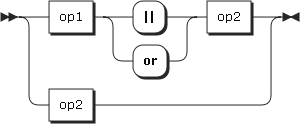
\includegraphics[scale=0.49]{design/diagram/lop1.png} 
\captionof{figure}{Gramática or lógico }
\end{center}
\end{multicols}

\paragraph{And lógico}
\begin{multicols}{2}
\begin{lstlisting}[style=nonumbers]      
op2 ::=  op2 ( "&&" | "and" ) op3
      |  op3
\end{lstlisting}  
\columnbreak	
\begin{center}
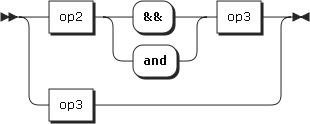
\includegraphics[scale=0.49]{design/diagram/op2.png} 
\captionof{figure}{Gramática and lógico}
\end{center}
\end{multicols}

\paragraph{Negación lógica}
\begin{multicols}{2}
\begin{lstlisting}[style=nonumbers]      
op3 ::=  "!" op3 
      |  op4
\end{lstlisting}  
\columnbreak	
\begin{center}
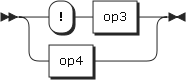
\includegraphics[scale=0.49]{design/diagram/op3.png} 
\captionof{figure}{Gramática negación lógica}
\end{center}
\end{multicols}

\paragraph{Comparaciones}
\begin{multicols}{2}
\begin{lstlisting}[style=nonumbers]      
op4 ::=  op4 "<" op5
      |  op4 "<=" op5
      |  op4 ">" op5
      |  op4 ">=" op5
      |  op4 "==" op5
      |  op4 "!=" op5
      |  op4 "===" op5
      |  op4 "!==" op5
      |  op5
\end{lstlisting}  
\columnbreak	
\begin{center}
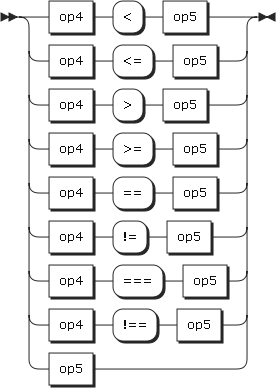
\includegraphics[scale=0.42]{design/diagram/op4.png} 
\captionof{figure}{Gramática comparaciones}
\end{center}
\end{multicols}

\subsubsection{Operadores aritméticos}
\paragraph{Suma y diferencia}
\begin{multicols}{2}
\begin{lstlisting}[style=nonumbers]      
op5 ::= op5 "+" op6
      |  op5  "-" op6
      |  op6
\end{lstlisting}  
\columnbreak	
\begin{center}
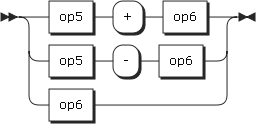
\includegraphics[scale=0.5]{design/diagram/op5.png} 
\captionof{figure}{Gramática operadores aritméticos}
\end{center}
\end{multicols}

\paragraph{Producto y división}
\begin{multicols}{2}
\begin{lstlisting}[style=nonumbers]      
op6  ::= op6 "*" op7
      |  op6 "/" op7
      |  op7
\end{lstlisting}  
\columnbreak	
\begin{center}
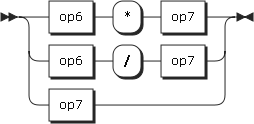
\includegraphics[scale=0.5]{design/diagram/op6.png} 
\captionof{figure}{Gramática producto y división}
\end{center}
\end{multicols}

\paragraph{Potencia y módulo}
\begin{multicols}{2}
\begin{lstlisting}[style=nonumbers]      
op7  ::= op7 "^" op8
      |  op7 "%" op8
      |  op8
\end{lstlisting}  
\columnbreak	
\begin{center}
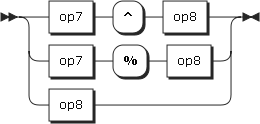
\includegraphics[scale=0.5]{design/diagram/op7.png} 
\captionof{figure}{Gramática potencia y módulo}
\end{center}
\end{multicols}

\subsubsection{Operadores cadenas de caracteres}
\paragraph{Concatenación}
\begin{multicols}{2}
\begin{lstlisting}[style=nonumbers]      
op8 ::=  op8 "." op9
      |  op9
\end{lstlisting}  
\columnbreak	
\begin{center}
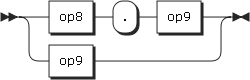
\includegraphics[scale=0.5]{design/diagram/op8.png} 
\captionof{figure}{Gramática operadores cadenas de caracteres}
\end{center}
\end{multicols}
\paragraph{Flujo}
\begin{multicols}{2}
\begin{lstlisting}[style=nonumbers]      
op9  ::= call "<<" op9
      |  call
\end{lstlisting}  
\columnbreak	
\begin{center}
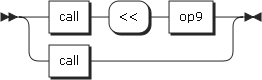
\includegraphics[scale=0.5]{design/diagram/op9.png} 
\captionof{figure}{Gramática flujo}
\end{center}
\end{multicols}

\subsubsection{Llamadas}
\begin{multicols}{2}
\begin{lstlisting}[style=nonumbers]      
call ::= call "(" list? ")"
      |  opc
\end{lstlisting}  
\columnbreak	
\begin{center}
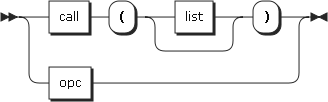
\includegraphics[scale=0.5]{design/diagram/call.png} 
\captionof{figure}{Gramática llamadas}
\end{center}
\end{multicols}

\subsubsection{Operadores condicionales}
\begin{multicols}{2}
\begin{lstlisting}[style=nonumbers]      
opc ::=  tern
      |  nullcoalescing
      |  unity
\end{lstlisting}  
\columnbreak	
\begin{center}
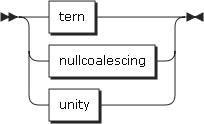
\includegraphics[scale=0.5]{design/diagram/opc.png} 
\captionof{figure}{Gramática operadores condicionales}
\end{center}
\end{multicols}
\paragraph{Operador ternario}
\begin{multicols}{2}
\begin{lstlisting}[style=nonumbers]      
tern ::= exp "?" exp? ":" exp
   |  exp "?" exp
\end{lstlisting}  
\columnbreak	
\begin{center}
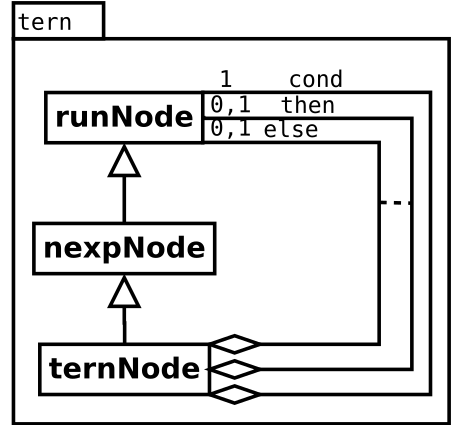
\includegraphics[scale=0.5]{design/diagram/tern.png} 
\captionof{figure}{Gramática operador ternario}
\end{center}
\end{multicols}
\paragraph{Null coalescing}
\begin{multicols}{2}
\begin{lstlisting}[style=nonumbers]      
nullcoalescing ::= "[[" list "]]"
\end{lstlisting}  
\columnbreak	
\begin{center}

\includegraphics[scale=0.5]{design/diagram/nullcoalescing.png} 
\captionof{figure}{Gramática fusión de nulos}
\end{center}
\end{multicols}

\pagebreak
\subsubsection{Operadores unitarios}
\begin{multicols}{2}
\begin{lstlisting}[style=nonumbers]      
unity ::=   inc_dec
         |  assignation_exp
         |  cast
         |  logical_func
         |  arith_func
         |  array_func
         |  string_func
         |  regexp_func
         |  iloop_access
         |  class_exp
         |  func_exp
         |  file
         |  date
         |  process
         |  generator
         |  environments
         |  array
         |  identity
\end{lstlisting}  
\columnbreak	
\begin{center}
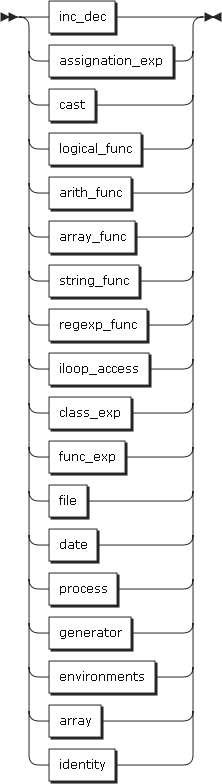
\includegraphics[scale=0.5]{design/diagram/unity.png} 
\captionof{figure}{Gramática operadores unitarios}
\end{center}
\end{multicols}

\paragraph{Incrementos y decrementos}
\begin{multicols}{2}
\begin{lstlisting}[style=nonumbers]      
inc_dec ::= "++" exp
         |  exp "++"
         |  "--" exp
         |  exp "--"
\end{lstlisting}  
\columnbreak	
\begin{center}
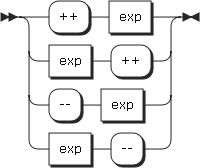
\includegraphics[scale=0.5]{design/diagram/inc_dec.png} 
\captionof{figure}{Gramática incrementos y decrementos}
\end{center}
\end{multicols}
\pagebreak
\paragraph{Conversión de tipos}
\begin{multicols}{2}
\begin{lstlisting}[style=nonumbers]      
cast ::= "int" exp
      |  "float" exp
      |  "bool" exp
      |  "str" exp
\end{lstlisting}  
\columnbreak	
\begin{center}
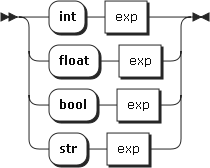
\includegraphics[scale=0.5]{design/diagram/cast.png} 
\captionof{figure}{Gramática conversión de tipos}
\end{center}
\end{multicols}



\paragraph{Accesos}
\begin{multicols}{2}
\begin{lstlisting}[style=nonumbers, basicstyle=\tiny]      
access ::=  access "->" id
         |  access "[" exp? "]"
         |  call "->" id
         |  call "[" exp? "]"
\end{lstlisting}  
\columnbreak	
\begin{center}
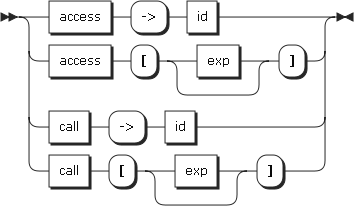
\includegraphics[scale=0.4]{design/diagram/access.png} 
\captionof{figure}{Gramática accesos}
\end{center}
\end{multicols}

\subsubsection{Asignaciones}
\begin{multicols}{2}
\begin{lstlisting}[style=nonumbers, basicstyle=\tiny]      
assignation ::=   
 (id | assignation | access)  "=" "&"? exp
\end{lstlisting}  
\columnbreak	
\begin{center}
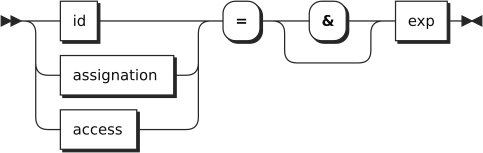
\includegraphics[scale=0.5]{design/diagram/assignation.png} 
\captionof{figure}{Gramática asignaciones}
\end{center}
\end{multicols}
\subsubsection{Funciones}
\begin{lstlisting}[style=nonumbers]
function ::= "~" id "(" params_val? ")" "{" stmts? "}"
\end{lstlisting}
\begin{center}
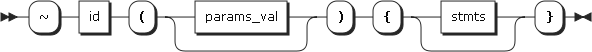
\includegraphics[scale=0.5]{design/diagram/function.png} 
\captionof{figure}{Gramática funciones}
\end{center}
\pagebreak

\paragraph {Función lambda}
\begin{lstlisting}[style=nonumbers]
function_lambda ::= "~" "(" params_val? ")" "{" stmts? "}"
    | "~" params_val ":" exp
    | "~&" id
\end{lstlisting}
\begin{center}
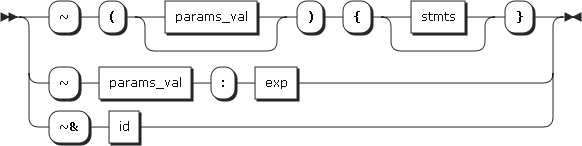
\includegraphics[scale=0.5]{design/diagram/function_lambda.png} 
\captionof{figure}{Gramática función lambda}
\end{center}
\paragraph {Cálculo parcial}
\begin{lstlisting}[style=nonumbers]
function_partial ::= "P" "[" params_val "]" "(" id ")"
   |  "P" "[" params_val "]" "(" function_exp ")"
   |  "P" "[" params_val "]" "(" arrayexp ")"
\end{lstlisting}
\begin{center}
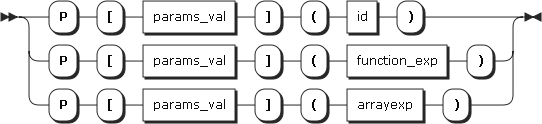
\includegraphics[scale=0.5]{design/diagram/function_partial.png} 
\captionof{figure}{Gramática función parcial}
\end{center}
\paragraph {Función de contexto}
\begin{lstlisting}[style=nonumbers]
function_context ::= "~>"
\end{lstlisting}
\begin{center}

\includegraphics[scale=0.5]{design/diagram/function_context.png} 
\captionof{figure}{Gramática función de contexto}
\end{center}


\subsubsection{Decoradores}
\begin{lstlisting}[style=nonumbers]
decorator ::= "~~" id "(" params_val? ")" "{" stmts? "}"
\end{lstlisting}
\begin{center}
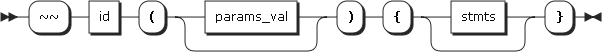
\includegraphics[scale=0.5]{design/diagram/decorator.png} 
\captionof{figure}{Gramática decoradores}
\end{center}
\paragraph{Decorador lambda}
\begin{lstlisting}[style=nonumbers]
decorator_lambda ::= "~~" "(" params_val? ")" "{" stmts? "}"
\end{lstlisting}
\begin{center}
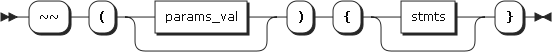
\includegraphics[scale=0.5]{design/diagram/function_decorator.png} 
\captionof{figure}{Gramática decorador lambda}
\end{center}

\subsubsection{Operadores clases y objetos}
\begin{multicols}{2}
\begin{lstlisting}[style=nonumbers]      
class_exp ::=  "new" id ("(" list? ")")?
            |  "this" 
            |  "parent"
            |  namespace
\end{lstlisting}  
\columnbreak	
\begin{center}
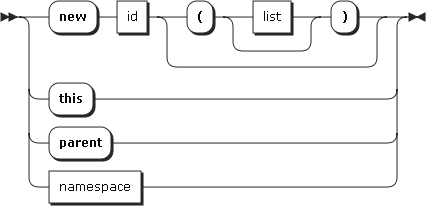
\includegraphics[scale=0.5]{design/diagram/class_exp.png} 
\captionof{figure}{Gramática operadores clases y objetos}
\end{center}
\end{multicols}

\subsubsection{Funciones del lenguaje}
\paragraph{Funciones lógicas}
\begin{multicols}{2}
\begin{lstlisting}[style=nonumbers]      
logical_func ::=  "isnull" exp
               |  "empty" exp
\end{lstlisting}  
\columnbreak	
\begin{center}
\includegraphics[scale=0.5]{design/diagram/logical_func.png} 
\captionof{figure}{Gramática funciones del lenguaje}
\end{center}
\end{multicols}

\paragraph{Funciones aritméticas}
\begin{multicols}{2}
\begin{lstlisting}[style=nonumbers]      
arith_func ::= "size" exp
            |  "sizeof" exp
\end{lstlisting}  
\columnbreak	
\begin{center}
\includegraphics[scale=0.5]{design/diagram/arith_func.png} 
\captionof{figure}{Gramática funciones aritméticas}
\end{center}
\end{multicols}
\pagebreak

\paragraph{Funciones cadenas de caracteres}
\begin{lstlisting}[style=nonumbers]      
string_func ::=   "sprintf" "(" exp "," exp ")"
               |  "str_replace" "(" exp "," exp "," exp ("," exp)? ")"
               |  "str_subreplace" "(" exp "," exp "," exp "," exp ")"
               |  "str_find" "(" exp "," exp ("," exp)? ")"
               |  "str_upper" "(" exp ")"
               |  "str_lower" "(" exp ")"
\end{lstlisting}  
\begin{center}
\includegraphics[scale=0.4]{design/diagram/string_func.png} 
\captionof{figure}{Gramática funciones cadenas de caracteres }
\end{center}

\paragraph{Funciones arrays}
\begin{multicols}{2}
\begin{lstlisting}[style=nonumbers]      
array_func ::= 
 "array_explode" "(" exp "," exp ")"
 |  "array_implode" "(" exp "," exp ")"
 |  "array_chunck" "(" exp "," exp ")"
 |  "array_reduce" "(" exp "," exp ")"
\end{lstlisting}  
\columnbreak	
\begin{center}
\includegraphics[scale=0.5]{design/diagram/array_func.png} 
\captionof{figure}{Gramática funciones array}
\end{center}
\end{multicols}

\paragraph{Funciones expresiones regulares}
\begin{lstlisting}[style=nonumbers]      
regexp_func ::=   "regexp" "(" exp ")"
               |  "search" "(" exp "," exp ("," list)? ")"
               |  "match" "(" exp "," exp ")"
\end{lstlisting}  
\begin{center}
\includegraphics[scale=0.5]{design/diagram/regexp_func.png} 
\captionof{figure}{Gramática funciones expresiones regulares}
\end{center}

\paragraph{Funciones fechas y tiempo}
\begin{multicols}{2}
\begin{lstlisting}[style=nonumbers]      
date ::= "date" "(" exp ")"
      |  "time" ("(" ")")
\end{lstlisting}  
\columnbreak	
\begin{center}
\includegraphics[scale=0.5]{design/diagram/date.png} 
\captionof{figure}{Gramática funciones  fechas y tiempo}
\end{center}
\end{multicols}

\paragraph{Funciones acceso a entorno}
\begin{multicols}{2}
\begin{lstlisting}[style=nonumbers]      
environment ::= "getenv" "(" exp ")"
\end{lstlisting}  
\columnbreak	
\begin{center}
\includegraphics[scale=0.4]{design/diagram/environment.png} 
\captionof{figure}{Gramática funciones acceso a entorno}
\end{center}
\end{multicols}

\paragraph{Funciones ficheros}
\begin{multicols}{2}
\begin{lstlisting}[style=nonumbers, basicstyle=\tiny]      
file ::= "file" "(" exp ("," exp)? ")"
   |  "fput" "(" exp "," exp ")"
   |  "fwrite" "(" exp "," exp ")"
   |  "fappend" "(" exp "," exp ")"
   |  "fget" "(" exp ("," exp)? ")"
   |  "fread" "(" exp ")"
   |  "fclose" "(" exp ")"
   |  "fseek" "(" exp "," exp ("," fposs)? ")"
   |  "ftell" "(" exp ")"

fpos ::= FSET
      |  FCUR
      |  FEND
\end{lstlisting}  
\begin{center}
\includegraphics[scale=0.4]{design/diagram/fpos.png} 
\captionof{figure}{Gramática fpos}
\end{center}
\columnbreak	
\begin{center}
\includegraphics[scale=0.4]{design/diagram/file.png} 
\captionof{figure}{Gramática file}
\end{center}
\end{multicols}
\pagebreak

\paragraph{Funciones procesos}
\begin{multicols}{2}
\begin{lstlisting}[style=nonumbers, basicstyle=\tiny]      
process ::= "exec" "(" exp ")"
         |  "eval" "(" exp ")"
         |  "fork" "(" ")"
         |  "wait" "(" exp? ")"
         |  "signal" "(" exp "," exp ")"
         |  "signalhandler" "(" exp "," exp ")"
         |  "exitProcess" "(" ")"
         |  "getpid" "(" ")"
         |  "getppid" "(" ")"
         |  "process" "(" exp ("," list)? ")"
\end{lstlisting}  
\columnbreak	
\begin{center}
\includegraphics[scale=0.4]{design/diagram/process.png} 
\captionof{figure}{Gramática funciones procesos}
\end{center}
\end{multicols}

\subsubsection{Generadores}
\begin{lstlisting}[style=nonumbers, basicstyle=\tiny]      
generator ::= "(" exp (":" exp)? "for" id (":" id )? "in" exp ( "if" exp )? ("{" stmts "}")? ")"
   | "(" exp (":" exp)? "for" "(" id (":" id )? "in" exp ")" ( "if" exp )? ("{" stmts "}")? ")"
\end{lstlisting}  
\begin{center}
\includegraphics[scale=0.4]{design/diagram/generator.png} 
\captionof{figure}{Gramática generadores}
\end{center}
% ----------------------------------------------------------------------
\subsection{Identidades}
\begin{multicols}{2}
\begin{lstlisting}[style=nonumbers]      
identity ::=   num
            |  "true"
            |  "false"
            |  "null"
            |  str
            |  rexp
            |  id 
\end{lstlisting}  
\columnbreak	
\begin{center}
\includegraphics[scale=0.4]{design/diagram/identity.png} 
\captionof{figure}{Gramática identidades}
\end{center}
\end{multicols}
\subsubsection{Parámetros}
\begin{lstlisting}[style=nonumbers]
params_val ::= params_val "," id "=" identity 
   |  params "," id "=" identity 
   |  id "=" identity 
   |  params
   
params ::= params "," "&"? id
   |  "&"? id
\end{lstlisting}
\begin{multicols}{2}
\begin{center}
\includegraphics[scale=0.4]{design/diagram/params_val.png} 
\captionof{figure}{Gramática valores de parámetros}
\end{center}
\columnbreak
\begin{center}
\includegraphics[scale=0.4]{design/diagram/params.png} 
\captionof{figure}{Gramática parámetros}
\end{center}
\end{multicols}

\subsubsection {Listas y pares}
\begin{multicols}{2}
\begin{lstlisting}[style=nonumbers]      
list ::= list "," exp?
      |  exp
\end{lstlisting}  
\begin{lstlisting}[style=nonumbers]      
map ::=  map "," pair?
      |  pair
   
pair ::= exp ":" exp
\end{lstlisting}  
\begin{center}
\includegraphics[scale=0.5]{design/diagram/pair.png} 
\captionof{figure}{Gramática pares}
\end{center}
\columnbreak	
\begin{center}
\includegraphics[scale=0.5]{design/diagram/list.png} 
\captionof{figure}{Gramática lista}
\end{center}
\begin{center}
\includegraphics[scale=0.5]{design/diagram/map.png} 
\captionof{figure}{Gramática diccionario}
\end{center}
\end{multicols}

\pagebreak
\subsubsection{Identificador}
\begin{multicols}{2}
\begin{lstlisting}[style=nonumbers]      
id ::= [a-zA-Z_][a-zA-Z0-9_]*
\end{lstlisting}  
\columnbreak	
\begin{center}
\includegraphics[scale=0.4]{design/diagram/id.png} 
\captionof{figure}{Gramática identificador}
\end{center}
\end{multicols}

\subsubsection{Números}
\begin{multicols}{2}
\begin{lstlisting}[style=nonumbers]      
num ::=  ("+"|"-"|) [0-9]+(.[0-9]+)?
\end{lstlisting}  
\columnbreak	
\begin{center}
\includegraphics[scale=0.5]{design/diagram/num.png} 
\captionof{figure}{Gramática números}
\end{center}
\end{multicols}
\subsubsection{Cadenas de caracteres}
\begin{multicols}{2}
\begin{lstlisting}[style=nonumbers]      
str ::= "'".* "'"
\end{lstlisting}  
\columnbreak	
\begin{center}
\includegraphics[scale=0.4]{design/diagram/str.png} 
\captionof{figure}{Gramática cadena de caracteres}
\end{center}
\end{multicols}

\subsubsection{Array}
\begin{multicols}{2}
\begin{lstlisting}[style=nonumbers]      
array ::=   "{" list "}"
         |  "{" map "}"
         |  "{""}"
         |  "arrayop"
         |  access
\end{lstlisting}  
\columnbreak	
\begin{center}
\includegraphics[scale=0.4]{design/diagram/array.png} 
\captionof{figure}{Gramática array}
\end{center}
\end{multicols}
\pagebreak

\subsubsection{Expresión regular}
\begin{multicols}{2}
\begin{lstlisting}[style=nonumbers]      
regexp ::= "`".*"`" 
\end{lstlisting}  
\columnbreak	
\begin{center}
\includegraphics[scale=0.4]{design/diagram/regexp.png} 
\captionof{figure}{Gramática expresión regular}
\end{center}
\end{multicols}

\subsubsection{Comentarios}
\begin{multicols}{2}
\begin{lstlisting}[style=nonumbers]      
comments ::=   "/*" [^*]* "*/"
            |  "//"[^\n]
            |  "#" [^#]
\end{lstlisting}  
\columnbreak	
\begin{center}
\includegraphics[scale=0.4]{design/diagram/comments.png} 
\captionof{figure}{Gramática comentarios}
\end{center}
\end{multicols}

% ======================================================================
\section{Diseño de comunicaciones}
OMI puede ser ejecutado de forma que guarde en un fichero una estructura de datos que representa el proceso de interpretación seguido. 
Esta estructura de datos tiene un formato JSON. En esta sección se presenta la estructura de estos ficheros mediante el esquema de 
json-schema.org.

Cuando el intérprete se ejecuta en modo servidor se vale de esta misma estructura para devolver el estado del proceso. Otros sistemas
que hagan de cliente pueden interpretar esta estructura de datos para operar con los mismos. 
% ======================================================================
\subsection{Esquema JSON}

\subsubsection{Nodos ejecutables}
La primera estructura de datos JSON que es guardada representa el árbol fruto del análisis léxico y sintáctico. Esta estructura de datos tiene como elemento
base un nodo que mantendrá relaciones con otros nodos. A partir del nodo raíz se puede obtener todo el árbol de nodos.


\begin{lstlisting}[language=omi]
{
   "$schema": "http://omi-project.com/json-schema/node",
   "title": "Nodos del |{\color{red}\emph{á}}|rbol sint|{\color{red}\emph{á}}|ctico"
   "type": "object",
   "properties": {
      "id": {
        "description": "Posici|{\color{red}\emph{ó}}|n de memoria del nodo",
        "type" : "string", 
      },
      "name": {
         "description": "Nombre del nodo",
         "type": "string",
      },
      "type": {
         "description": "Tipo del nodo",
         "type": "string",
      },
      "size": {
         "description": "Tama|{\color{red}\emph{ñ}}|o del nodo en Bytes",
         "type": "string",
      },
      "rel": {
         "description": "Relaciones con otros nodos",
         "type": "array",
         "items": {
            "ref":  "http://omi-project.com/json-schema/node"
         }
      },
      "relname": {
         "description": "Nombre de las relaciones con otros nodos",
         "type": "array",
         "items": {
            "type":  "string",
         }
      },
   }
}
\end{lstlisting}
\captionof{lstlisting}{JSON nodos ejecutables}

\subsubsection{Acciones}
Para representar el proceso de interpretación se precisa de una estructura de datos que indique las acciones 
llevadas a cabo en el proceso.

\begin{lstlisting}[language=omi]
{
   "$schema": "http://omi-project.com/json-schema/process",
   "title": "Proceso de interpretaci|{\color{red}\emph{ó}}|n",
   "type": "array",
   "items": {
      "type": "object",
        "properties": { 
            "action": {
               "description": "Acci|{\color{red}\emph{ó}}|n que se corresponde con un paso",
               "type": "enum",
            },
            "id": {
               "description": "Id del nodo sobre el que se lleva a cabo la acci|{\color{red}\emph{ó}}|n",
               "type": "string",
            },
            "attrs": {
               "description": "Atributos de la acci|{\color{red}\emph{ó}}|n. Dependen de la acci|{\color{red}\emph{ó}}|n".
               "type": "object",
            }
      }
   }
}
\end{lstlisting}
\captionof{lstlisting}{JSON acciones}

Los tipos de acciones son los siguientes:
\begin{description}
\item[run:] Ejecución de un nodo.
\item [runClass:] Ejecución de un nodo clase.
\item[endClass:] Finaliza la ejecución de una clase.
\item[setParent:] Establece el padre de un nodo clase.
\item[setValue:] Establece el valor de un nodo.
\item[setRef:] Establece el valor de una referencia.
\item[accessVar:] Accede al valor de una variable.
\item[accessFunc:] Accede al valor de una funcion.
\item[accessClass:] Accede al valor de una clase.
\item[clone:] Clona un nodo.
\item[newNode:] Crea un nuevo nodo.
\item[changeRef:] Cambia el valor de una referencia.
\item[changeValue:] Cambia el valor de un nodo.
\item[delete:] Elimina un nodo.
\item[print:] Imprime en la salida estándar.
\item[input:] Toma valores de la entrada estándar.
\item[toSymbols:] Añade elementos a la tabla de símbolos interna de un nodo.
\item[removeLevel:] Elimina un nivel de la tabla de símbolos.
\item[return:] Se devuelve un valor.
\item[error:] Se ha producido un error.
\item[sleep:] Se espera un evento.
\item[runStatic:] Comienza la ejecución de un elemento estático.
\item[endStatic:] Finaliza la ejecución de un elemento estático.
\item[runPrivate:] Comienza la ejecución de un elemento privado.
\item[endPrivate:] Finaliza la ejecución de un elemento privado.
\item[runGlobal:] Comienza la ejecución de un elemento global.
\item[endGlobal:] Finaliza la ejecución de un elemento global.
\item[line:] Especifica la línea actual del código fuente.
\end{description}



% ======================================================================
\section{Diseño de componentes}
Esta sección constituye el modelo de comportamiento básico.
Detalla cómo los distintos objetos interaccionan y se comunican entre sí para
analizar la entrada del usuario, correspondiente al código fuente, e interpretarlo
para su ejecución.

Se presenta un diagrama de secuencia para la operación interpretación
de un código fuente. Luego se presenta diagramas de comunicación correspondientes
a algunas sentencias escritas en el lenguaje.


% ======================================================================
\subsection{Interpretar código fuente}
Para la interpretación de código fuente el sistema crea los objetos 
encargados del análisis léxico y sintáctico del mismo. El objeto principal
del sistema se encarga de crear e inicializar el analizador sintáctico (parser) a
partir del código fuente, a su vez este crea el analizador léxico (scanner)
que crea una estructura correspondiente al código fuente que será interpretado.\\

El sistema envía un mensaje para que el parser analice el código fuente.
El analizador sintáctico define una serie de reglas gramaticales e irá comprobando que 
el código fuente cumple estas reglas a la vez que las utiliza para crear un árbol de derivación 
denominado árbol sintáctico. Para ello hace uso de una serie de tokens que irá solicitando 
al analizador léxico. Este último obtendrá los tokens a partir del código fuente, mediante 
una serie de reglas léxicas formadas a partir de lenguajes regulares. \\


Por cada regla gramatical que se cumpla en el parser, este habrá obtenido del scanner tantos tokens como 
componentes léxicos sean necesarios para cumplir la regla. 

\begin{multicols}{2}
Además por cada regla gramatical se construirá un nodo ejecutable formado a partir del valor asociado a una serie de tokens, o 
a partir de otros nodos ejecutables construidos por reglas de mayor prioridad y creados en 
anteriores interacciones. Esto formará un árbol sintáctico formado por nodos ejecutables que 
contienen la semántica que encierran las construcciones del código fuente.\\

A partir del nodo raíz del árbol de nodos ejecutables comienza un recorrido en profundidad del
árbol que conllevará la ejecución del código fuente, produciéndose así el resultado semántico 
esperado.\\

En el caso de que no se de una regla gramatical que se corresponda con el código analizado se 
producirá un error sintáctico. Por otro lado, en el caso de que alguna cadena contenida
en el código fuente no se corresponda con los lenguajes regulares que define el scanner
se producirá un error léxico.

\columnbreak 
\begin{center}
\includegraphics[scale=0.17]{design/interaction.png} 
\captionof{figure}{Interacción interpretar código fuente}
\end{center}
\end{multicols}

\subsection{Sentencias}
%~ \subsubsection {Sentencia de control condicional }
\begin{center}
\includegraphics[scale=0.38]{design/if_componentes.png} 
\captionof{figure}{Objetos sentencia condicional}
\end{center}

%~ \subsubsection {Operaciones aritméticas }
\begin{center}
\includegraphics[scale=0.38]{design/arith.png} 
\captionof{figure}{Objetos operaciones aritméticas }
\end{center}

%~ \subsubsection {Asignaciones }
\begin{center}
\includegraphics[scale=0.38]{design/asig.png} 
\captionof{figure}{Objetos asignaciones}
\end{center}

\begin{center}
\includegraphics[scale=0.38]{design/asig2.png} 
\captionof{figure}{Objetos asignaciones (2)}
\end{center}

\begin{center}
\includegraphics[scale=0.38]{design/asig3.png} 
\captionof{figure}{Objetos asignaciones (3)}
\end{center}

% ----------------------------------------------------------------------
% ======================================================================
\section{Diseño de la interfaz de usuario}
En esta sección se describe el diseño de la interfaz del usuario a partir del análisis llevado a cabo.

El intérprete presenta una interfaz de consola de comandos, por lo que el diseño se corresponde con una descripción de los usos 
del comando y el listado de las opciones que acepta.

El cliente runTree y la web en general presenta una interfaz web. El diseño se corresponde con una descripción 
gráfica de las páginas que la conforman y de las secciones que las componen.
% ======================================================================
\subsection{Intérprete}
El intérprete es un programa de consola de comando por lo que la interfaz con el usuario no es gráfica.

El comando ``omi'' permite ejecutar el intérprete. Se puede usar de las siguientes forma:
\begin{itemize}
   \item omi [opciones] $<fichero>$ [argumentos...]
   \item omi -c $<codigo>$ [argumentos...]
   \item omi -i [argumentos...]
   \item omi -sj $<fichero.json>$
\end{itemize}

El listado de opciones que acepta el comando a continuación:

\begin{description}
\item[-i	]:	Ejecuta el intérprete de forma interactiva.
 \item [-c $<codigo>$]:	Interpreta el código dado.
 \item [-l $<fichero.so>$]: Carga el módulo $<fichero.so>$.
\item [-h]: Muestra la ayuda.
 \item[-V]: Muestra la versión.
\item [-j $<fichero.json>$]: Imprime una descripción del procesos en formato json en el fichero $<fichero.json>$.
  \item [-x $<pasos>$]: Obtiene $<pasos>$ pasos del proceso de interpretación en cada petición. 
 \item [-s]:	Ejecuta como servidor en el puerto 8888.
\end {description}

% ======================================================================
\subsection{runTree}

runTree es un cliente web del intérprete OMI. Muestra información sobre el proceso de interpretación y permite navegar por este. 

El sistema lo compone una única página web con un diseño de cuadrícula.

\begin{center}
\includegraphics[scale=0.2]{design/runtree.png} 
\captionof{figure}{Interfaz de usuario runTree}
\end{center}

La primera parte de la retícula, superior izquierda, muestra el árbol sintáctico correspondiente al código enviado. En este árbol se marcarán los nodos a medida 
que se van ejecutando y resolviendo semánticamente, mostrando información directa de cada nodo como el nombre, el valor o el tipo.
En la segunda parte, superior derecha, muestra las tablas de símbolos de variables, funciones y clases. Esta sección permite navegar por las tablas de símbolos 
y los elementos que serán referenciados desde las mismas.

En la tercera parte, inferior izquierda, se muestra el código fuente y la interfaz de entrada/salida del programa.

En la última sección, inferior derecha, se muestra una consola informativa, en la que aparece una descripción del nodo actualmente en ejecución o 
los nodos seleccionados por el usuario. También se colocan en esta sección las opciones de control para avanzar un paso, una sentencia, la reproducción automática, abrir un fichero local o guardar el 
código en un fichero local. 

\subsection{Sitio web}
Según el análisis de la interfaz de usuario llevado a cabo se procede a detallar gráficamente cada página descrita.

%~ \subsubsection{Home}
\begin{center}
\includegraphics[scale=0.1]{design/home.png} 
\captionof{figure}{Interfaz de usuario home}
\end{center}

%~ \subsubsection{Sobre OMI}
\begin{center}
\includegraphics[scale=0.1]{design/about.png} 
\captionof{figure}{Interfaz de usuario sobre OMI}
\end{center}

%~ \subsubsection{Contacto}
\begin{center}
\includegraphics[scale=0.1]{design/contact.png} 
\captionof{figure}{Interfaz de usuario contacto}
\end{center}

%~ \subsubsection{Índice de la documentación}
\begin{center}
\includegraphics[scale=0.1]{design/doc-index.png} 
\captionof{figure}{Interfaz de usuario índice de la documentación}
\end{center}

%~ \subsubsection{Documento}
\begin{center}
\includegraphics[scale=0.1]{design/doc-content-x.png} 
\captionof{figure}{Interfaz de usuario documento}
\end{center}

%~ \subsubsection{Navegador de gramática}
\begin{center}
\includegraphics[scale=0.1]{design/gramatic-x.png} 
\captionof{figure}{Interfaz de usuario navegador de gramática}
\end{center}

%~ \subsubsection{Navegador de clases}
\begin{center}
\includegraphics[scale=0.1]{design/class.png} 
\captionof{figure}{Interfaz de usuario navegador de clases}
\end{center}

%~ \subsubsection{Navegador de ficheros}
\begin{center}
\includegraphics[scale=0.1]{design/files.png} 
\captionof{figure}{Interfaz de usuario navegador de ficheros}
\end{center}

%~ \subsubsection{Descargas}
\begin{center}
\includegraphics[scale=0.1]{design/download.png} 
\captionof{figure}{Interfaz de usuario descargas}
\end{center}


